%% Author: 青木貴弘
\subsection{未知の突発天体の探査} \label{transients.s3.unknowns}
{ %% Localize settings
\newcommand{\suffix}[2]{^{> #1 \, \text{mJy}} _{#2 \, \text{GHz}}}
\newcommand{\ntt}{那須 20~m 電波望遠鏡}
\newcommand{\WJN}{WJN J1443+3439}
\newcommand{\FDR}{{\it FDR}}
\newcommand{\siglevel}{\mbox{$10^{-5}$}~}
\newcommand{\ssd}{天球面密度}

%% Body
%%
%% ss1
%%
\subsubsection{従来の探査結果}
他の波長域で対応天体が見つからないような、未知の突発天体の探査が何度か行われてきている。
例えば\citet{2002ApJ...576..923L}は orphan GRB afterglow をカタログ比較によって探査し、9つの候補天体を発見した。
その後、追観測やデータの再解析によって8つが偽陽性検出であることが判明し、1つについては電波のみを放射しているII型超新星とわかりVLA~121550.2+130654 と命名された \citep{2006ApJ...639..331G,2010ApJ...711..517O}。

それ以降、未知の突発天体探査が活発化し、それらの探査結果を図示したものが\Figref{fig:transients.s3.unknowns.rate}である。
図中の各プロットは脚注に示す文献に基づいている\footnote{
\Figref{fig:transients.s3.unknowns.rate}の各プロットは次の文献をもとにしている: \citealt{2007ApJ...666..346B} (Bow07 2-month/single), \citealt{2010ApJ...725.1792B} (Bow10a/b), \citealt{2011ApJ...740...65O} (Ofe11), \citealt{2012AJ....143...96J} (Jae12), \citealt{2006ApJ...639..331G} (Gal06), \citealt{2011MNRAS.412..634B} (Ban11), \citealt{2010ApJ...719...45C} (Cro10),  \citealt{2011ApJ...728L..14B} (Bow11a/b), \citealt{2014ApJ...781...10A} (Aok14), \citealt{2010AJ....140.1995L} (Laz10)。
いくつかのプロットは\citet{2011MNRAS.415....2B}, \citet{2012ApJ...747...70F}にまとめられている。
}。
\Figref{fig:transients.s3.unknowns.rate}の横軸は観測感度、つまり最小検出フラックス密度$S$を表し、縦軸は天球上の単位面積を観測したときに、フラックス密度が$S$を超える未知天体を発見できる個数、つまり天球面上の個数密度$\varSigma (>S)$を表す。
この天球面上の個数密度 (sky-surface density) はスナップショットレート (snapshot rate) とも呼ばれ、イメージング観測の結果として導くことができる発見確率の指標であり、この量をイベントレートに換算することができる。
\begin{figure}
	\centering
	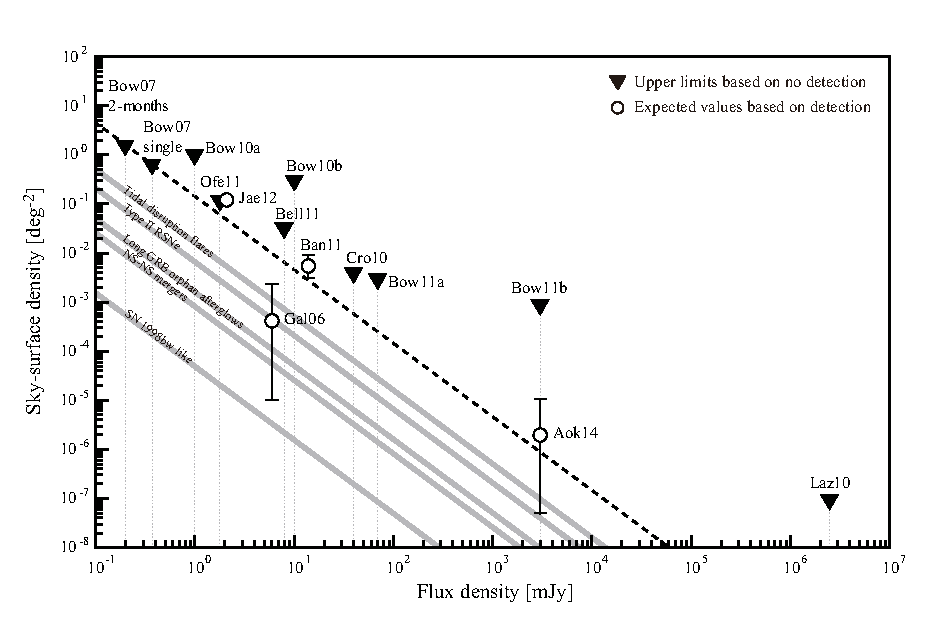
\includegraphics[width=1\textwidth]{transients/transients.s3.unknowns.rate.eps}
	\caption{未知の突発天体に対する、天球面上の個数密度$\varSigma (>S)$ とフラックス密度 $S$ の関係 \citep{2014ApJ...781...10A}。
	ただし観測周波数は考慮していない。
	三角形のプロットは突発天体が発見されなかった探査結果を示し、円形のプロットはいくつかの発見があった探査結果を示す。
	灰色の太線は\citet{2012ApJ...747...70F}によって推定された、既知天体の個数密度を表している。}
	\label{fig:transients.s3.unknowns.rate}
\end{figure}%

これらの探査によって、いくつかの候補天体が発見されてきているが、その起源のみならず発見の真偽についても確証は得られていない。
この検証のためには、従来の観測装置の性能では多くの観測時間が必要となり現実的ではなく、SKAによる広視野・高感度な探査観測が必要となる。
そこで、これらの検証のためにSKAに必要な性能を、早稲田大学の那須電波観測所による探査結果を例にして提案する。

%%
%% ss2
%%
\subsubsection{従来の探査結果の検証}
\paragraph{検証の方法}
\Figref{fig:transients.s3.unknowns.rate}の Aok14 というプロットは、那須電波観測所 (\Figref{fig:transients.s3.gw.nasu}) で行った突発天体の探査結果を示している。
その探査では、1日程度の継続時間をもつ起源不明の突発天体を発見し、\WJN と命名した \citep{2007ApJ...657L..37N}。
この発見から、周波数1.42 GHzにおいてフラックス密度3000~mJy以上を持つ未知の突発天体の個数密度は、$\varSigma \suffix{3000}{1.42} = 2^{+9}_{-1.9} \times 10^{-6}~\persqdeg$ と見積もられる\footnote{
\citet{2010ApJ...711..517O}の定義に従えばイベントレート $\mathfrak{R}$ は個数密度$\varSigma$と光度変動の継続時間$W$を用いて$\mathfrak{R} = \varSigma / W$で与えられ、那須電波観測所で発見されたWJNイベントに対しては$%
	\mathfrak{R}\suffix{3000}{1.42} = 7^{+33}_{-7} \times 10^{-4}(W/\text{day})^{-1} \persqdeg \peryr 
	= 30^{+136}_{-28} (W/\text{day})^{-1} \persky \peryr%
$
を得る。
単位 sky は全天$4\pi~\text{sr}$として定義した。
}。
したがって任意のフラックス密度$S$における個数密度は
\begin{equation}
	\varSigma^{>S}_{\text{1.42~GHz}} = 0.3~\persqdeg \times \left(  S/\text{mJy} \right)^{-3/2}
	\label{eq:transients.s3.unknowns.nasu-dens}
\end{equation}
で推定できる。
この観測結果の正当性は、広い面積を高い感度で探査することによって検証が可能である。
\Eqref{eq:transients.s3.unknowns.nasu-dens}という結果を検証するために必要な、探査観測の感度$S$と掃天面積$\varOmega$の関係は、統計的な議論によって\footnote{
突発現象の生起個数はポアソン過程であるから事象の生起間隔 $\varOmega$ は指数分布となり、突発天体を発見できる確率は$P(\varOmega)=1-\e^{-\varSigma \varOmega}$で与えられる。
このとき95\% 以上の確率で少なくとも一つの天体を発見するために必要な掃天面積$\varOmega$ は$P(\varOmega) \leq 95\%$で与えられる。
}
\begin{equation}
	\varOmega / \sqdeg > 10 \times \left( S/\text{mJy} \right)^{+3/2}
	\label{eq:transients.s3.unknowns.survey-config}
\end{equation}
で与えられる \citep{2014ApJ...781...10A}。
この関係を満たす観測を行えば95\% の確率で同様の突発天体を検出できるはずであり、もし検出できなければ\Eqref{eq:transients.s3.unknowns.nasu-dens}という観測結果は棄却されうることになる。
このようにして那須電波観測所による探査結果のみならず、\Figref{fig:transients.s3.unknowns.rate}に示す従来の結果の多くを検証することができる。

\paragraph{検証のためのSKAへの要求}
SKA Phase 1 を用いて\Eqref{eq:transients.s3.unknowns.survey-config}を満たす観測を行えば、従来の探査結果を検証することができる。
%装置要求をするにあたり、既にデザインされている性能パラメーターのいくつかを固定し、アンテナ台数と受信機冷却に関係するパラメーター、実効開口面積$A_\text{e}$とシステム雑音温度$T_\text{sys}$を不定として、感度パラメーター$A_\text{e}/T_\text{sys}$に対する要求を述べる。
GHz帯域で行われてきた従来の探査を検証するという観点からは、必要になるのは\skamid{} または \skasur{} のアンテナであり、突発天体探査で最も重要な要素は視野の広さであるから、\skasur{}が最も適したアンテナといえる。
そこで主に\skasur{1}アンテナの基本デザインをもとに、検証に必要な system equivalent flux density (SEFD) を考える。

\skasur{1} アンテナには phased array feed (PAF) とよばれるフィードが搭載される予定であり、既存のASKAPの周波数帯域を考えると、SKA1で最初に実装するのは PAF Band~2 (周波数650--1670~MHz、視野 $18~\sqdeg$) が妥当だろう。
また観測可能な帯域幅は片偏波あたり最大500~MHzとされている。
最小検出フラックスを$S_\text{min}=\text{SEFD}_\text{array}/(\eta_\text{s}\sqrt{\varDelta \nu \ \tau})$とし検出閾値を$S=7S_\text{min}$とすると、\Eqref{eq:transients.s3.unknowns.survey-config}を満たすようなSEFDは
\begin{align}
	\text{SEFD}_\text{array} 
	< 260~\text{Jy} \times \left( \frac{\varOmega}{18~\sqdeg} \right)^{2/3}
		\cdot \frac{\eta_\text{s}}{0.9} \cdot 
		\sqrt{\frac{\varDelta \nu}{500~\text{MHz}} \cdot \frac{\tau}{1~\text{hour}}}
	%&= 15~\text{Jy} \cdot \left( \frac{\varOmega}{18~\sqdeg} \right)^{2/3}
	%	\cdot \frac{\eta_\text{s}}{0.9} \cdot 
	%	\sqrt{\frac{\varDelta \nu}{100~\text{MHz}} \cdot \frac{\tau}{1~\text{min}}}
		\label{eq:transients.s3.unknowns.sefd}
\end{align}
となる\footnote{\Eqref{eq:transients.s3.unknowns.sefd}は\skasur{1}の性能を単位としているが、当然\skamid{1}への要求検討にも使用できる。}。
ここで$\eta_\text{s}$はシステム効率、$\varDelta \nu$は観測帯域幅、$\tau$は積分時間を表す。
SKAの基本的な性能はおおよそ固まっているため、例えば建設するべきアンテナの台数に着目すると、現状の単一鏡のデザイン $\text{SEFD}_\text{dish}=586~\text{Jy}$ が実現するとすれば、上記の検証観測をするには{\ 感度のみの観点からは}3台で事足りる\footnote{$\text{SEFD}_\text{array} \simeq \text{SEFD}_\text{dish}/m$, $m=\text{アンテナの台数}$。}。
ただしもちろんこの見積もりは、光度変動のタイムスケールが1時間以上の突発天体に対するものである。

\WJN の継続時間は4分以上3日以内としか制限されておらず、またGCRT J1745-3009 のように数分スケールの電波変動を起こす天体を観測しようとすると (\Secref{transients.s1.unknowns})、上記の見積もりではその観測は実現できない。
また500~MHzという帯域幅は使用可能な上限値であり、実際の観測ではより狭帯域に制限されることもありうる。
そのような状況を考え、帯域幅100~MHzを積分時間1~minで観測することを考えると$\text{SEFD}_\text{array}=15~\text{Jy}$が必要になり、その場合アンテナは40台必要になる。
ただし\skasur{1} の計画では60台のアンテナを建設予定であり\footnote{\skasur{1}アンテナ60台、ASKAPアンテナ36台で計96台のアンテナを運用することも計画されているが、本節の見積もりにASKAPアンテナは含めていない。}、$\text{SEFD}_\text{array}=10~\text{Jy}$を得られるから、上記の検証観測は十分に実施可能である。
積分時間が1~minという観測では$u$--$v$平面の埋まりが悪いが、\Figref{fig:transients.phasespace}の中央付近の空白領域を埋めることにつながり、未知の突発天体の探査には重要な時間分解能である。

\subsubsection{未知の探査}

%既に理論的に存在することは知られているが実際に観測されたことはない、あるいは数例の観測例はあるものの確証が得られていない天体、つまり\Secref{transients.s2.wilkinson}で述べた「既知の未知 (known unknowns)」の探査をすることが、今後の電波天文学にとって重要である。
%この点について、SKAは他の電波望遠鏡に比べて極めて強いアドバンテージを持っており、その探査をすることは宇宙科学にブレイクスルーを起こせる数少ない手段の一つである。

未知の天体の例としては、\Secref{transients.s1}や\Figref{fig:transients.s3.unknowns.rate}にも示した潮汐崩壊現象や orphan GRB afterglow などがあり、前者は Swift J1644+57 という観測例があるが詳細はわかっておらず、後者は観測例もない。
これらを能動的に探査することがSKAには求められ、実際に発見するために必要な性能をSKAに持たせなければならない。
そこでここでは、\skasur{1}による探査と発見のための要求性能を考える。


\citet{2012ApJ...747...70F}の見積もりによれば\Figref{fig:transients.s3.unknowns.rate}の斜線に示したように、可視光放射がないII型電波超新星 \citep{2006ApJ...639..331G} の個数密度は$\varSigma^{>S} = 6.6\times 10^{-3}~\persqdeg \times (S/\text{mJy})^{-3/2}$である。
このレートを単位にして、電波帯域における突発天体を95\% 以上の確率で発見するために必要な観測は、
\begin{align}
	\biggl( \frac{\text{SEFD}_\text{array}}{10~\text{Jy}} \biggr)^{-2}
	\biggl( \frac{\varOmega}{18~\sqdeg} \biggr)^{4/3} 
	\biggl( \frac{\eta_\text{s}}{0.9} \biggr)^2 \cdot 
	\frac{\varDelta \nu}{500~\text{MHz}} \cdot \frac{\tau}{6~\text{hour}}
	> 0.041
	\label{eq:transients.s3.unknowns.SNII}
\end{align}
という関係を満たすような観測設定をする必要がある\footnote{$\text{SEFD}_\text{dish} = 586~\text{Jy}$のSKAアンテナ60台で干渉計を構成すると、$\text{SEFD}_\text{array} = 10~\text{Jy}$を得る。}。
したがって、例えば15分程度の観測をするだけで、従来数々の電波望遠鏡を駆使してようやく発見した、可視光対応天体のないII型超新星を95\% の確率で発見できるということである。

しかし一方で、Ic型極超新星SN 1998bw (GRB 980425) と同様の突発天体を探査しようとすると、個数密度が$\varSigma^{>S} = 4.9\times 10^{-5}~\persqdeg \times (S/\text{mJy})^{-3/2}$でありイベントレートが低すぎるため、電波帯域だけで探査しようとすると約180時間の観測時間が必要となる。
これを実現するには、約1か月間に渡って受信機性能を安定化させ、かつデータ較正をするシステムが必要になるだろう。

\subsubsection{まとめ}

従来さまざまな電波望遠鏡を用いて、未知の突発天体が探査されてきているが、視野の広さと感度の高さが両立した観測は難しく、効果的な探査は行われてこなかった。
SKAはこの現状を打破し、とりわけ\skasur{} は広い視野、高い感度、高い空間分解能を同時に実現し、突発天体研究にとって強力なツールとなるだろう。
単に従来の探査結果を検証するだけならば、\skasur{1} アンテナの台数は5台もあれば可能だが、それでは理論的に予測されているが実観測例のない orphan GRB afterglow や Ia 型超新星の研究を行うことができない。
したがって現状のデザインを実現することが重要である。
そしてその探査が実現すれば、まだ観測例のない突発天体も容易に発見できると見積もられる。




} %% End of localization
